\documentclass[1p]{elsarticle_modified}
%\bibliographystyle{elsarticle-num}

%\usepackage[colorlinks]{hyperref}
%\usepackage{abbrmath_seonhwa} %\Abb, \Ascr, \Acal ,\Abf, \Afrak
\usepackage{amsfonts}
\usepackage{amssymb}
\usepackage{amsmath}
\usepackage{amsthm}
\usepackage{scalefnt}
\usepackage{amsbsy}
\usepackage{kotex}
\usepackage{caption}
\usepackage{subfig}
\usepackage{color}
\usepackage{graphicx}
\usepackage{xcolor} %% white, black, red, green, blue, cyan, magenta, yellow
\usepackage{float}
\usepackage{setspace}
\usepackage{hyperref}

\usepackage{tikz}
\usetikzlibrary{arrows}

\usepackage{multirow}
\usepackage{array} % fixed length table
\usepackage{hhline}

%%%%%%%%%%%%%%%%%%%%%
\makeatletter
\renewcommand*\env@matrix[1][\arraystretch]{%
	\edef\arraystretch{#1}%
	\hskip -\arraycolsep
	\let\@ifnextchar\new@ifnextchar
	\array{*\c@MaxMatrixCols c}}
\makeatother %https://tex.stackexchange.com/questions/14071/how-can-i-increase-the-line-spacing-in-a-matrix
%%%%%%%%%%%%%%%

\usepackage[normalem]{ulem}

\newcommand{\msout}[1]{\ifmmode\text{\sout{\ensuremath{#1}}}\else\sout{#1}\fi}
%SOURCE: \msout is \stkout macro in https://tex.stackexchange.com/questions/20609/strikeout-in-math-mode

\newcommand{\cancel}[1]{
	\ifmmode
	{\color{red}\msout{#1}}
	\else
	{\color{red}\sout{#1}}
	\fi
}

\newcommand{\add}[1]{
	{\color{blue}\uwave{#1}}
}

\newcommand{\replace}[2]{
	\ifmmode
	{\color{red}\msout{#1}}{\color{blue}\uwave{#2}}
	\else
	{\color{red}\sout{#1}}{\color{blue}\uwave{#2}}
	\fi
}

\newcommand{\Sol}{\mathcal{S}} %segment
\newcommand{\D}{D} %diagram
\newcommand{\A}{\mathcal{A}} %arc


%%%%%%%%%%%%%%%%%%%%%%%%%%%%%5 test

\def\sl{\operatorname{\textup{SL}}(2,\Cbb)}
\def\psl{\operatorname{\textup{PSL}}(2,\Cbb)}
\def\quan{\mkern 1mu \triangleright \mkern 1mu}

\theoremstyle{definition}
\newtheorem{thm}{Theorem}[section]
\newtheorem{prop}[thm]{Proposition}
\newtheorem{lem}[thm]{Lemma}
\newtheorem{ques}[thm]{Question}
\newtheorem{cor}[thm]{Corollary}
\newtheorem{defn}[thm]{Definition}
\newtheorem{exam}[thm]{Example}
\newtheorem{rmk}[thm]{Remark}
\newtheorem{alg}[thm]{Algorithm}

\newcommand{\I}{\sqrt{-1}}
\begin{document}

%\begin{frontmatter}
%
%\title{Boundary parabolic representations of knots up to 8 crossings}
%
%%% Group authors per affiliation:
%\author{Yunhi Cho} 
%\address{Department of Mathematics, University of Seoul, Seoul, Korea}
%\ead{yhcho@uos.ac.kr}
%
%
%\author{Seonhwa Kim} %\fnref{s_kim}}
%\address{Center for Geometry and Physics, Institute for Basic Science, Pohang, 37673, Korea}
%\ead{ryeona17@ibs.re.kr}
%
%\author{Hyuk Kim}
%\address{Department of Mathematical Sciences, Seoul National University, Seoul 08826, Korea}
%\ead{hyukkim@snu.ac.kr}
%
%\author{Seokbeom Yoon}
%\address{Department of Mathematical Sciences, Seoul National University, Seoul, 08826,  Korea}
%\ead{sbyoon15@snu.ac.kr}
%
%\begin{abstract}
%We find all boundary parabolic representation of knots up to 8 crossings.
%
%\end{abstract}
%\begin{keyword}
%    \MSC[2010] 57M25 
%\end{keyword}
%
%\end{frontmatter}

%\linenumbers
%\tableofcontents
%
\newcommand\colored[1]{\textcolor{white}{\rule[-0.35ex]{0.8em}{1.4ex}}\kern-0.8em\color{red} #1}%
%\newcommand\colored[1]{\textcolor{white}{ #1}\kern-2.17ex	\textcolor{white}{ #1}\kern-1.81ex	\textcolor{white}{ #1}\kern-2.15ex\color{red}#1	}

{\Large $\underline{12n_{0493}~(K12n_{0493})}$}

\setlength{\tabcolsep}{10pt}
\renewcommand{\arraystretch}{1.6}
\vspace{1cm}\begin{tabular}{m{100pt}>{\centering\arraybackslash}m{274pt}}
\multirow{5}{120pt}{
	\centering
	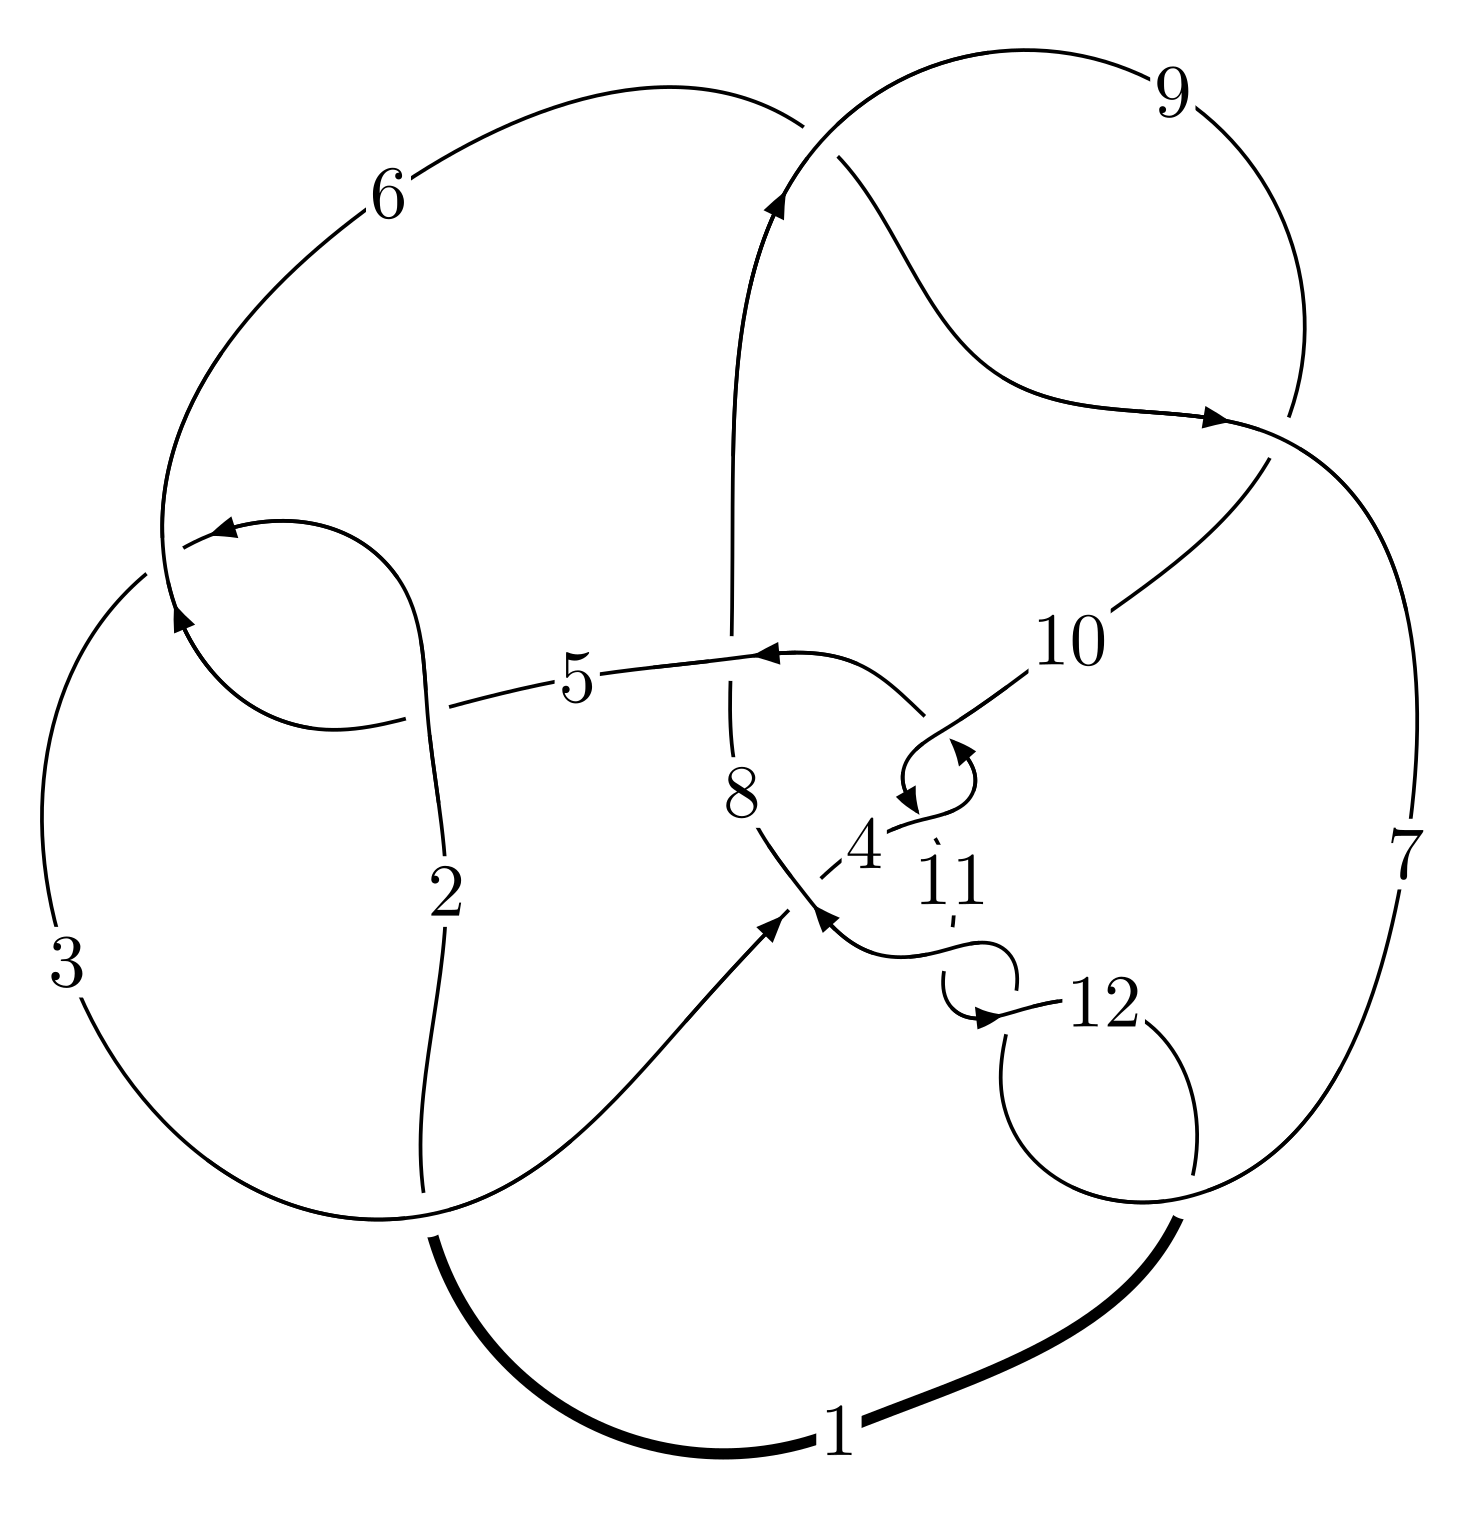
\includegraphics[width=112pt]{../../../GIT/diagram.site/Diagrams/png/2582_12n_0493.png}\\
\ \ \ A knot diagram\footnotemark}&
\allowdisplaybreaks
\textbf{Linearized knot diagam} \\
\cline{2-2}
 &
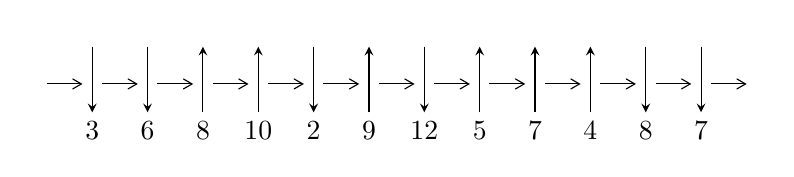
\begin{tikzpicture}[x=20pt, y=17pt]
	% nodes
	\node (C0) at (0, 0) {};
	\node (C1) at (1, 0) {};
	\node (C1U) at (1, +1) {};
	\node (C1D) at (1, -1) {3};

	\node (C2) at (2, 0) {};
	\node (C2U) at (2, +1) {};
	\node (C2D) at (2, -1) {6};

	\node (C3) at (3, 0) {};
	\node (C3U) at (3, +1) {};
	\node (C3D) at (3, -1) {8};

	\node (C4) at (4, 0) {};
	\node (C4U) at (4, +1) {};
	\node (C4D) at (4, -1) {10};

	\node (C5) at (5, 0) {};
	\node (C5U) at (5, +1) {};
	\node (C5D) at (5, -1) {2};

	\node (C6) at (6, 0) {};
	\node (C6U) at (6, +1) {};
	\node (C6D) at (6, -1) {9};

	\node (C7) at (7, 0) {};
	\node (C7U) at (7, +1) {};
	\node (C7D) at (7, -1) {12};

	\node (C8) at (8, 0) {};
	\node (C8U) at (8, +1) {};
	\node (C8D) at (8, -1) {5};

	\node (C9) at (9, 0) {};
	\node (C9U) at (9, +1) {};
	\node (C9D) at (9, -1) {7};

	\node (C10) at (10, 0) {};
	\node (C10U) at (10, +1) {};
	\node (C10D) at (10, -1) {4};

	\node (C11) at (11, 0) {};
	\node (C11U) at (11, +1) {};
	\node (C11D) at (11, -1) {8};

	\node (C12) at (12, 0) {};
	\node (C12U) at (12, +1) {};
	\node (C12D) at (12, -1) {7};
	\node (C13) at (13, 0) {};

	% arrows
	\draw[->,>={angle 60}]
	(C0) edge (C1) (C1) edge (C2) (C2) edge (C3) (C3) edge (C4) (C4) edge (C5) (C5) edge (C6) (C6) edge (C7) (C7) edge (C8) (C8) edge (C9) (C9) edge (C10) (C10) edge (C11) (C11) edge (C12) (C12) edge (C13) ;	\draw[->,>=stealth]
	(C1U) edge (C1D) (C2U) edge (C2D) (C3D) edge (C3U) (C4D) edge (C4U) (C5U) edge (C5D) (C6D) edge (C6U) (C7U) edge (C7D) (C8D) edge (C8U) (C9D) edge (C9U) (C10D) edge (C10U) (C11U) edge (C11D) (C12U) edge (C12D) ;
	\end{tikzpicture} \\
\hhline{~~} \\& 
\textbf{Solving Sequence} \\ \cline{2-2} 
 &
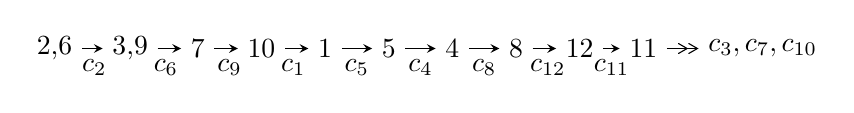
\begin{tikzpicture}[x=23pt, y=7pt]
	% node
	\node (A0) at (-1/8, 0) {2,6};
	\node (A1) at (17/16, 0) {3,9};
	\node (A2) at (17/8, 0) {7};
	\node (A3) at (25/8, 0) {10};
	\node (A4) at (33/8, 0) {1};
	\node (A5) at (41/8, 0) {5};
	\node (A6) at (49/8, 0) {4};
	\node (A7) at (57/8, 0) {8};
	\node (A8) at (65/8, 0) {12};
	\node (A9) at (73/8, 0) {11};
	\node (C1) at (1/2, -1) {$c_{2}$};
	\node (C2) at (13/8, -1) {$c_{6}$};
	\node (C3) at (21/8, -1) {$c_{9}$};
	\node (C4) at (29/8, -1) {$c_{1}$};
	\node (C5) at (37/8, -1) {$c_{5}$};
	\node (C6) at (45/8, -1) {$c_{4}$};
	\node (C7) at (53/8, -1) {$c_{8}$};
	\node (C8) at (61/8, -1) {$c_{12}$};
	\node (C9) at (69/8, -1) {$c_{11}$};
	\node (A10) at (11, 0) {$c_{3},c_{7},c_{10}$};

	% edge
	\draw[->,>=stealth]	
	(A0) edge (A1) (A1) edge (A2) (A2) edge (A3) (A3) edge (A4) (A4) edge (A5) (A5) edge (A6) (A6) edge (A7) (A7) edge (A8) (A8) edge (A9) ;
	\draw[->>,>={angle 60}]	
	(A9) edge (A10);
\end{tikzpicture} \\ 

\end{tabular} \\

\footnotetext{
The image of knot diagram is generated by the software ``\textbf{Draw programme}" developed by Andrew Bartholomew(\url{http://www.layer8.co.uk/maths/draw/index.htm\#Running-draw}), where we modified some parts for our purpose(\url{https://github.com/CATsTAILs/LinksPainter}).
}\phantom \\ \newline 
\centering \textbf{Ideals for irreducible components\footnotemark of $X_{\text{par}}$} 
 
\begin{align*}
I^u_{1}&=\langle 
-5.43760\times10^{104} u^{68}+2.00230\times10^{105} u^{67}+\cdots+1.22634\times10^{105} b-1.11649\times10^{106},\\
\phantom{I^u_{1}}&\phantom{= \langle  }4.64010\times10^{105} u^{68}-1.59745\times10^{106} u^{67}+\cdots+1.34897\times10^{106} a+7.48313\times10^{106},\\
\phantom{I^u_{1}}&\phantom{= \langle  }u^{69}-4 u^{68}+\cdots+56 u-11\rangle \\
I^u_{2}&=\langle 
10 u^{22}+5 u^{21}+\cdots+b-13,\;5 u^{22}+2 u^{21}+\cdots+a-3,\;u^{23}+u^{22}+\cdots- u-1\rangle \\
\\
\end{align*}
\raggedright * 2 irreducible components of $\dim_{\mathbb{C}}=0$, with total 92 representations.\\
\footnotetext{All coefficients of polynomials are rational numbers. But the coefficients are sometimes approximated in decimal forms when there is not enough margin.}
\newpage
\renewcommand{\arraystretch}{1}
\centering \section*{I. $I^u_{1}= \langle -5.44\times10^{104} u^{68}+2.00\times10^{105} u^{67}+\cdots+1.23\times10^{105} b-1.12\times10^{106},\;4.64\times10^{105} u^{68}-1.60\times10^{106} u^{67}+\cdots+1.35\times10^{106} a+7.48\times10^{106},\;u^{69}-4 u^{68}+\cdots+56 u-11 \rangle$}
\flushleft \textbf{(i) Arc colorings}\\
\begin{tabular}{m{7pt} m{180pt} m{7pt} m{180pt} }
\flushright $a_{2}=$&$\begin{pmatrix}1\\0\end{pmatrix}$ \\
\flushright $a_{6}=$&$\begin{pmatrix}0\\u\end{pmatrix}$ \\
\flushright $a_{3}=$&$\begin{pmatrix}1\\u^2\end{pmatrix}$ \\
\flushright $a_{9}=$&$\begin{pmatrix}-0.343973 u^{68}+1.18420 u^{67}+\cdots+17.5685 u-5.54728\\0.443401 u^{68}-1.63275 u^{67}+\cdots-32.3170 u+9.10424\end{pmatrix}$ \\
\flushright $a_{7}=$&$\begin{pmatrix}-0.576164 u^{68}+1.77245 u^{67}+\cdots+24.1892 u-5.92136\\-0.358276 u^{68}+0.999822 u^{67}+\cdots+13.4977 u-3.58010\end{pmatrix}$ \\
\flushright $a_{10}=$&$\begin{pmatrix}0.494384 u^{68}-1.74440 u^{67}+\cdots-36.5327 u+8.98958\\0.165294 u^{68}-0.478041 u^{67}+\cdots-7.38945 u+2.38124\end{pmatrix}$ \\
\flushright $a_{1}=$&$\begin{pmatrix}- u^2+1\\- u^4\end{pmatrix}$ \\
\flushright $a_{5}=$&$\begin{pmatrix}u\\u\end{pmatrix}$ \\
\flushright $a_{4}=$&$\begin{pmatrix}1.10192 u^{68}-3.35873 u^{67}+\cdots-47.8714 u+14.8013\\0.0132321 u^{68}-0.00521372 u^{67}+\cdots+5.24343 u-0.0882060\end{pmatrix}$ \\
\flushright $a_{8}=$&$\begin{pmatrix}-0.311783 u^{68}+1.36760 u^{67}+\cdots+27.5302 u-9.20533\\0.475591 u^{68}-1.44935 u^{67}+\cdots-22.3553 u+5.44619\end{pmatrix}$ \\
\flushright $a_{12}=$&$\begin{pmatrix}0.842075 u^{68}-3.29112 u^{67}+\cdots-71.9419 u+20.0300\\-0.344233 u^{68}+0.630033 u^{67}+\cdots-6.87988 u+4.46895\end{pmatrix}$ \\
\flushright $a_{11}=$&$\begin{pmatrix}-0.829938 u^{68}+1.76140 u^{67}+\cdots-4.47063 u+5.32558\\-1.27286 u^{68}+3.52866 u^{67}+\cdots+35.8363 u-4.75348\end{pmatrix}$\\&\end{tabular}
\flushleft \textbf{(ii) Obstruction class $= -1$}\\~\\
\flushleft \textbf{(iii) Cusp Shapes $= 3.43232 u^{68}-10.6390 u^{67}+\cdots-136.515 u+28.1198$}\\~\\
\newpage\renewcommand{\arraystretch}{1}
\flushleft \textbf{(iv) u-Polynomials at the component}\newline \\
\begin{tabular}{m{50pt}|m{274pt}}
Crossings & \hspace{64pt}u-Polynomials at each crossing \\
\hline $$\begin{aligned}c_{1}\end{aligned}$$&$\begin{aligned}
&u^{69}+36 u^{68}+\cdots+474 u+121
\end{aligned}$\\
\hline $$\begin{aligned}c_{2},c_{5}\end{aligned}$$&$\begin{aligned}
&u^{69}+4 u^{68}+\cdots+56 u+11
\end{aligned}$\\
\hline $$\begin{aligned}c_{3}\end{aligned}$$&$\begin{aligned}
&u^{69}+u^{68}+\cdots+29817 u+6379
\end{aligned}$\\
\hline $$\begin{aligned}c_{4},c_{10}\end{aligned}$$&$\begin{aligned}
&u^{69}+3 u^{68}+\cdots-1049 u+701
\end{aligned}$\\
\hline $$\begin{aligned}c_{6},c_{9}\end{aligned}$$&$\begin{aligned}
&u^{69}-3 u^{68}+\cdots+55 u+193
\end{aligned}$\\
\hline $$\begin{aligned}c_{7},c_{11},c_{12}\end{aligned}$$&$\begin{aligned}
&u^{69}+2 u^{68}+\cdots+13 u-1
\end{aligned}$\\
\hline $$\begin{aligned}c_{8}\end{aligned}$$&$\begin{aligned}
&u^{69}- u^{68}+\cdots+395 u-29
\end{aligned}$\\
\hline
\end{tabular}\\~\\
\newpage\renewcommand{\arraystretch}{1}
\flushleft \textbf{(v) Riley Polynomials at the component}\newline \\
\begin{tabular}{m{50pt}|m{274pt}}
Crossings & \hspace{64pt}Riley Polynomials at each crossing \\
\hline $$\begin{aligned}c_{1}\end{aligned}$$&$\begin{aligned}
&y^{69}+8 y^{68}+\cdots-141470 y-14641
\end{aligned}$\\
\hline $$\begin{aligned}c_{2},c_{5}\end{aligned}$$&$\begin{aligned}
&y^{69}-36 y^{68}+\cdots+474 y-121
\end{aligned}$\\
\hline $$\begin{aligned}c_{3}\end{aligned}$$&$\begin{aligned}
&y^{69}+81 y^{68}+\cdots-1405779003 y-40691641
\end{aligned}$\\
\hline $$\begin{aligned}c_{4},c_{10}\end{aligned}$$&$\begin{aligned}
&y^{69}+77 y^{68}+\cdots-18986053 y-491401
\end{aligned}$\\
\hline $$\begin{aligned}c_{6},c_{9}\end{aligned}$$&$\begin{aligned}
&y^{69}-33 y^{68}+\cdots+199499 y-37249
\end{aligned}$\\
\hline $$\begin{aligned}c_{7},c_{11},c_{12}\end{aligned}$$&$\begin{aligned}
&y^{69}+20 y^{68}+\cdots+9 y-1
\end{aligned}$\\
\hline $$\begin{aligned}c_{8}\end{aligned}$$&$\begin{aligned}
&y^{69}-23 y^{68}+\cdots+200453 y-841
\end{aligned}$\\
\hline
\end{tabular}\\~\\
\newpage\flushleft \textbf{(vi) Complex Volumes and Cusp Shapes}
$$\begin{array}{c|c|c}  
\text{Solutions to }I^u_{1}& \I (\text{vol} + \sqrt{-1}CS) & \text{Cusp shape}\\
 \hline 
\begin{aligned}
u &= -0.290552 + 0.976534 I \\
a &= \phantom{-}0.662659 + 1.042150 I \\
b &= -0.021606 + 0.325176 I\end{aligned}
 & \phantom{-}3.93320 - 4.10094 I & \phantom{-0.000000 -}0. + 7.59043 I \\ \hline\begin{aligned}
u &= -0.290552 - 0.976534 I \\
a &= \phantom{-}0.662659 - 1.042150 I \\
b &= -0.021606 - 0.325176 I\end{aligned}
 & \phantom{-}3.93320 + 4.10094 I & \phantom{-0.000000 } 0. - 7.59043 I \\ \hline\begin{aligned}
u &= \phantom{-}0.170915 + 1.016760 I \\
a &= \phantom{-}0.735038 - 0.888007 I \\
b &= -0.122632 + 0.149326 I\end{aligned}
 & -3.69662 + 2.16087 I & \phantom{-0.000000 } 0 \\ \hline\begin{aligned}
u &= \phantom{-}0.170915 - 1.016760 I \\
a &= \phantom{-}0.735038 + 0.888007 I \\
b &= -0.122632 - 0.149326 I\end{aligned}
 & -3.69662 - 2.16087 I & \phantom{-0.000000 } 0 \\ \hline\begin{aligned}
u &= \phantom{-}0.845794 + 0.445199 I \\
a &= \phantom{-}1.042270 - 0.541687 I \\
b &= \phantom{-}1.05454 - 1.32366 I\end{aligned}
 & \phantom{-}1.75302 + 0.23405 I & \phantom{-}2.64178 + 0. I\phantom{ +0.000000I} \\ \hline\begin{aligned}
u &= \phantom{-}0.845794 - 0.445199 I \\
a &= \phantom{-}1.042270 + 0.541687 I \\
b &= \phantom{-}1.05454 + 1.32366 I\end{aligned}
 & \phantom{-}1.75302 - 0.23405 I & \phantom{-}2.64178 + 0. I\phantom{ +0.000000I} \\ \hline\begin{aligned}
u &= \phantom{-}0.798359 + 0.685065 I \\
a &= \phantom{-}1.103240 - 0.280353 I \\
b &= \phantom{-}0.552794 - 0.298714 I\end{aligned}
 & \phantom{-}2.19476 + 0.59175 I & \phantom{-0.000000 } 0 \\ \hline\begin{aligned}
u &= \phantom{-}0.798359 - 0.685065 I \\
a &= \phantom{-}1.103240 + 0.280353 I \\
b &= \phantom{-}0.552794 + 0.298714 I\end{aligned}
 & \phantom{-}2.19476 - 0.59175 I & \phantom{-0.000000 } 0 \\ \hline\begin{aligned}
u &= -0.611426 + 0.705280 I \\
a &= \phantom{-}0.834581 + 0.752090 I \\
b &= -0.413709 - 0.331884 I\end{aligned}
 & \phantom{-}6.87382 + 1.62388 I & \phantom{-}8.32922 - 2.64435 I \\ \hline\begin{aligned}
u &= -0.611426 - 0.705280 I \\
a &= \phantom{-}0.834581 - 0.752090 I \\
b &= -0.413709 + 0.331884 I\end{aligned}
 & \phantom{-}6.87382 - 1.62388 I & \phantom{-}8.32922 + 2.64435 I\\
 \hline 
 \end{array}$$\newpage$$\begin{array}{c|c|c}  
\text{Solutions to }I^u_{1}& \I (\text{vol} + \sqrt{-1}CS) & \text{Cusp shape}\\
 \hline 
\begin{aligned}
u &= -0.673306 + 0.638312 I \\
a &= -1.45289 - 0.49248 I \\
b &= -0.339907 + 0.110846 I\end{aligned}
 & \phantom{-}2.72164 - 0.99882 I & \phantom{-0.000000 } 0. - 1.55232 I \\ \hline\begin{aligned}
u &= -0.673306 - 0.638312 I \\
a &= -1.45289 + 0.49248 I \\
b &= -0.339907 - 0.110846 I\end{aligned}
 & \phantom{-}2.72164 + 0.99882 I & \phantom{-0.000000 -}0. + 1.55232 I \\ \hline\begin{aligned}
u &= \phantom{-}0.828451 + 0.406795 I \\
a &= \phantom{-}1.37279 - 0.90899 I \\
b &= \phantom{-}0.076668 - 0.891427 I\end{aligned}
 & \phantom{-}1.87674 - 3.82550 I & \phantom{-0.000000 -}0. + 7.69744 I \\ \hline\begin{aligned}
u &= \phantom{-}0.828451 - 0.406795 I \\
a &= \phantom{-}1.37279 + 0.90899 I \\
b &= \phantom{-}0.076668 + 0.891427 I\end{aligned}
 & \phantom{-}1.87674 + 3.82550 I & \phantom{-0.000000 } 0. - 7.69744 I \\ \hline\begin{aligned}
u &= -1.011290 + 0.463825 I \\
a &= -0.817036 - 1.011240 I \\
b &= -1.21636 - 1.85408 I\end{aligned}
 & \phantom{-}1.46489 + 5.12150 I & \phantom{-0.000000 } 0 \\ \hline\begin{aligned}
u &= -1.011290 - 0.463825 I \\
a &= -0.817036 + 1.011240 I \\
b &= -1.21636 + 1.85408 I\end{aligned}
 & \phantom{-}1.46489 - 5.12150 I & \phantom{-0.000000 } 0 \\ \hline\begin{aligned}
u &= -1.048530 + 0.378591 I \\
a &= \phantom{-}0.491834 - 0.900948 I \\
b &= \phantom{-}0.00957 - 1.57580 I\end{aligned}
 & -2.49072 + 3.79882 I & \phantom{-0.000000 } 0 \\ \hline\begin{aligned}
u &= -1.048530 - 0.378591 I \\
a &= \phantom{-}0.491834 + 0.900948 I \\
b &= \phantom{-}0.00957 + 1.57580 I\end{aligned}
 & -2.49072 - 3.79882 I & \phantom{-0.000000 } 0 \\ \hline\begin{aligned}
u &= \phantom{-}0.398655 + 1.050660 I \\
a &= -0.931521 + 0.797871 I \\
b &= \phantom{-}0.157270 + 0.032104 I\end{aligned}
 & -2.97736 + 9.69199 I & \phantom{-0.000000 } 0 \\ \hline\begin{aligned}
u &= \phantom{-}0.398655 - 1.050660 I \\
a &= -0.931521 - 0.797871 I \\
b &= \phantom{-}0.157270 - 0.032104 I\end{aligned}
 & -2.97736 - 9.69199 I & \phantom{-0.000000 } 0\\
 \hline 
 \end{array}$$\newpage$$\begin{array}{c|c|c}  
\text{Solutions to }I^u_{1}& \I (\text{vol} + \sqrt{-1}CS) & \text{Cusp shape}\\
 \hline 
\begin{aligned}
u &= -0.843195 + 0.221726 I \\
a &= -0.93965 + 1.06792 I \\
b &= -0.52957 + 1.58476 I\end{aligned}
 & -1.18583 - 1.43148 I & \phantom{-}3.84710 - 6.37744 I \\ \hline\begin{aligned}
u &= -0.843195 - 0.221726 I \\
a &= -0.93965 - 1.06792 I \\
b &= -0.52957 - 1.58476 I\end{aligned}
 & -1.18583 + 1.43148 I & \phantom{-}3.84710 + 6.37744 I \\ \hline\begin{aligned}
u &= -0.592910 + 0.619767 I \\
a &= -1.42026 - 0.66221 I \\
b &= -0.267942 + 0.039618 I\end{aligned}
 & \phantom{-}2.72523 - 1.00845 I & \phantom{-}1.13200 - 1.33542 I \\ \hline\begin{aligned}
u &= -0.592910 - 0.619767 I \\
a &= -1.42026 + 0.66221 I \\
b &= -0.267942 - 0.039618 I\end{aligned}
 & \phantom{-}2.72523 + 1.00845 I & \phantom{-}1.13200 + 1.33542 I \\ \hline\begin{aligned}
u &= \phantom{-}0.937541 + 0.663875 I \\
a &= \phantom{-}0.369232 - 1.125340 I \\
b &= \phantom{-}0.23643 - 1.79333 I\end{aligned}
 & \phantom{-}1.73480 - 5.81339 I & \phantom{-0.000000 } 0 \\ \hline\begin{aligned}
u &= \phantom{-}0.937541 - 0.663875 I \\
a &= \phantom{-}0.369232 + 1.125340 I \\
b &= \phantom{-}0.23643 + 1.79333 I\end{aligned}
 & \phantom{-}1.73480 + 5.81339 I & \phantom{-0.000000 } 0 \\ \hline\begin{aligned}
u &= \phantom{-}1.095940 + 0.350670 I \\
a &= -0.474582 + 0.632682 I \\
b &= -1.72631 + 1.19121 I\end{aligned}
 & \phantom{-}3.07674 - 3.26894 I & \phantom{-0.000000 } 0 \\ \hline\begin{aligned}
u &= \phantom{-}1.095940 - 0.350670 I \\
a &= -0.474582 - 0.632682 I \\
b &= -1.72631 - 1.19121 I\end{aligned}
 & \phantom{-}3.07674 + 3.26894 I & \phantom{-0.000000 } 0 \\ \hline\begin{aligned}
u &= -1.081310 + 0.487072 I \\
a &= -0.659733 - 0.708574 I \\
b &= \phantom{-}0.62165 - 1.72240 I\end{aligned}
 & -7.58609 + 6.42641 I & \phantom{-0.000000 } 0 \\ \hline\begin{aligned}
u &= -1.081310 - 0.487072 I \\
a &= -0.659733 + 0.708574 I \\
b &= \phantom{-}0.62165 + 1.72240 I\end{aligned}
 & -7.58609 - 6.42641 I & \phantom{-0.000000 } 0\\
 \hline 
 \end{array}$$\newpage$$\begin{array}{c|c|c}  
\text{Solutions to }I^u_{1}& \I (\text{vol} + \sqrt{-1}CS) & \text{Cusp shape}\\
 \hline 
\begin{aligned}
u &= \phantom{-}1.105510 + 0.431642 I \\
a &= \phantom{-}1.004780 + 0.584794 I \\
b &= \phantom{-}0.26453 + 1.61847 I\end{aligned}
 & -7.94202 - 0.79088 I & \phantom{-0.000000 } 0 \\ \hline\begin{aligned}
u &= \phantom{-}1.105510 - 0.431642 I \\
a &= \phantom{-}1.004780 - 0.584794 I \\
b &= \phantom{-}0.26453 - 1.61847 I\end{aligned}
 & -7.94202 + 0.79088 I & \phantom{-0.000000 } 0 \\ \hline\begin{aligned}
u &= -1.147280 + 0.304107 I \\
a &= \phantom{-}0.550803 + 0.761091 I \\
b &= -0.31435 + 1.82784 I\end{aligned}
 & -9.68321 - 0.62268 I & \phantom{-0.000000 } 0 \\ \hline\begin{aligned}
u &= -1.147280 - 0.304107 I \\
a &= \phantom{-}0.550803 - 0.761091 I \\
b &= -0.31435 - 1.82784 I\end{aligned}
 & -9.68321 + 0.62268 I & \phantom{-0.000000 } 0 \\ \hline\begin{aligned}
u &= -0.993265 + 0.683955 I \\
a &= -0.282845 - 1.144910 I \\
b &= -0.76540 - 1.96652 I\end{aligned}
 & \phantom{-}1.75235 + 6.29447 I & \phantom{-0.000000 } 0 \\ \hline\begin{aligned}
u &= -0.993265 - 0.683955 I \\
a &= -0.282845 + 1.144910 I \\
b &= -0.76540 + 1.96652 I\end{aligned}
 & \phantom{-}1.75235 - 6.29447 I & \phantom{-0.000000 } 0 \\ \hline\begin{aligned}
u &= \phantom{-}1.207420 + 0.035311 I \\
a &= \phantom{-}0.069551 + 0.357262 I \\
b &= \phantom{-}0.526334 + 0.627810 I\end{aligned}
 & -2.81273 - 0.16209 I & \phantom{-0.000000 } 0 \\ \hline\begin{aligned}
u &= \phantom{-}1.207420 - 0.035311 I \\
a &= \phantom{-}0.069551 - 0.357262 I \\
b &= \phantom{-}0.526334 - 0.627810 I\end{aligned}
 & -2.81273 + 0.16209 I & \phantom{-0.000000 } 0 \\ \hline\begin{aligned}
u &= -1.033920 + 0.650381 I \\
a &= \phantom{-}0.381960 + 0.552392 I \\
b &= \phantom{-}1.18877 + 1.43009 I\end{aligned}
 & \phantom{-}5.59026 + 3.61321 I & \phantom{-0.000000 } 0 \\ \hline\begin{aligned}
u &= -1.033920 - 0.650381 I \\
a &= \phantom{-}0.381960 - 0.552392 I \\
b &= \phantom{-}1.18877 - 1.43009 I\end{aligned}
 & \phantom{-}5.59026 - 3.61321 I & \phantom{-0.000000 } 0\\
 \hline 
 \end{array}$$\newpage$$\begin{array}{c|c|c}  
\text{Solutions to }I^u_{1}& \I (\text{vol} + \sqrt{-1}CS) & \text{Cusp shape}\\
 \hline 
\begin{aligned}
u &= \phantom{-}1.117680 + 0.556781 I \\
a &= -0.890564 - 0.750983 I \\
b &= -0.37281 - 1.65828 I\end{aligned}
 & -7.95415 - 8.38570 I & \phantom{-0.000000 } 0 \\ \hline\begin{aligned}
u &= \phantom{-}1.117680 - 0.556781 I \\
a &= -0.890564 + 0.750983 I \\
b &= -0.37281 + 1.65828 I\end{aligned}
 & -7.95415 + 8.38570 I & \phantom{-0.000000 } 0 \\ \hline\begin{aligned}
u &= \phantom{-}1.085710 + 0.625989 I \\
a &= -0.503128 + 0.612693 I \\
b &= -0.287588 + 1.243300 I\end{aligned}
 & -1.07599 - 2.78600 I & \phantom{-0.000000 } 0 \\ \hline\begin{aligned}
u &= \phantom{-}1.085710 - 0.625989 I \\
a &= -0.503128 - 0.612693 I \\
b &= -0.287588 - 1.243300 I\end{aligned}
 & -1.07599 + 2.78600 I & \phantom{-0.000000 } 0 \\ \hline\begin{aligned}
u &= \phantom{-}0.798698 + 0.974655 I \\
a &= -0.432695 + 0.595898 I \\
b &= -0.166512 + 0.361764 I\end{aligned}
 & -0.24985 - 3.26069 I & \phantom{-0.000000 } 0 \\ \hline\begin{aligned}
u &= \phantom{-}0.798698 - 0.974655 I \\
a &= -0.432695 - 0.595898 I \\
b &= -0.166512 - 0.361764 I\end{aligned}
 & -0.24985 + 3.26069 I & \phantom{-0.000000 } 0 \\ \hline\begin{aligned}
u &= \phantom{-}0.319351 + 0.663934 I \\
a &= \phantom{-}1.11830 + 1.01941 I \\
b &= -0.155956 + 1.246900 I\end{aligned}
 & -5.68469 + 3.59684 I & \phantom{-}0.14375 - 2.17339 I \\ \hline\begin{aligned}
u &= \phantom{-}0.319351 - 0.663934 I \\
a &= \phantom{-}1.11830 - 1.01941 I \\
b &= -0.155956 - 1.246900 I\end{aligned}
 & -5.68469 - 3.59684 I & \phantom{-}0.14375 + 2.17339 I \\ \hline\begin{aligned}
u &= \phantom{-}0.961426 + 0.848715 I \\
a &= -0.426077 + 0.482317 I \\
b &= -0.077045 + 1.197380 I\end{aligned}
 & -0.94415 - 3.29961 I & \phantom{-0.000000 } 0 \\ \hline\begin{aligned}
u &= \phantom{-}0.961426 - 0.848715 I \\
a &= -0.426077 - 0.482317 I \\
b &= -0.077045 - 1.197380 I\end{aligned}
 & -0.94415 + 3.29961 I & \phantom{-0.000000 } 0\\
 \hline 
 \end{array}$$\newpage$$\begin{array}{c|c|c}  
\text{Solutions to }I^u_{1}& \I (\text{vol} + \sqrt{-1}CS) & \text{Cusp shape}\\
 \hline 
\begin{aligned}
u &= \phantom{-}0.687662 + 0.185413 I \\
a &= -1.79140 - 0.10939 I \\
b &= \phantom{-}0.487312 - 1.099210 I\end{aligned}
 & \phantom{-}4.79965 + 0.76507 I & -0.89012 - 1.45079 I \\ \hline\begin{aligned}
u &= \phantom{-}0.687662 - 0.185413 I \\
a &= -1.79140 + 0.10939 I \\
b &= \phantom{-}0.487312 + 1.099210 I\end{aligned}
 & \phantom{-}4.79965 - 0.76507 I & -0.89012 + 1.45079 I \\ \hline\begin{aligned}
u &= -1.196820 + 0.622088 I \\
a &= \phantom{-}0.667975 + 0.833159 I \\
b &= \phantom{-}0.97633 + 1.75198 I\end{aligned}
 & \phantom{-}1.19205 + 9.84022 I & \phantom{-0.000000 } 0 \\ \hline\begin{aligned}
u &= -1.196820 - 0.622088 I \\
a &= \phantom{-}0.667975 - 0.833159 I \\
b &= \phantom{-}0.97633 - 1.75198 I\end{aligned}
 & \phantom{-}1.19205 - 9.84022 I & \phantom{-0.000000 } 0 \\ \hline\begin{aligned}
u &= \phantom{-}1.258550 + 0.582507 I \\
a &= \phantom{-}0.452188 - 0.889836 I \\
b &= \phantom{-}1.10957 - 1.91755 I\end{aligned}
 & -7.04483 - 7.85806 I & \phantom{-0.000000 } 0 \\ \hline\begin{aligned}
u &= \phantom{-}1.258550 - 0.582507 I \\
a &= \phantom{-}0.452188 + 0.889836 I \\
b &= \phantom{-}1.10957 + 1.91755 I\end{aligned}
 & -7.04483 + 7.85806 I & \phantom{-0.000000 } 0 \\ \hline\begin{aligned}
u &= \phantom{-}1.213600 + 0.688126 I \\
a &= -0.517780 + 0.965581 I \\
b &= -1.02405 + 2.11674 I\end{aligned}
 & -5.5104 - 15.9437 I & \phantom{-0.000000 } 0 \\ \hline\begin{aligned}
u &= \phantom{-}1.213600 - 0.688126 I \\
a &= -0.517780 - 0.965581 I \\
b &= -1.02405 - 2.11674 I\end{aligned}
 & -5.5104 + 15.9437 I & \phantom{-0.000000 } 0 \\ \hline\begin{aligned}
u &= -0.499390 + 0.340618 I \\
a &= -0.919752 - 0.049244 I \\
b &= \phantom{-}0.05015 - 2.33868 I\end{aligned}
 & -5.61165 - 2.54761 I & \phantom{-}5.30359 + 0.02313 I \\ \hline\begin{aligned}
u &= -0.499390 - 0.340618 I \\
a &= -0.919752 + 0.049244 I \\
b &= \phantom{-}0.05015 + 2.33868 I\end{aligned}
 & -5.61165 + 2.54761 I & \phantom{-}5.30359 - 0.02313 I\\
 \hline 
 \end{array}$$\newpage$$\begin{array}{c|c|c}  
\text{Solutions to }I^u_{1}& \I (\text{vol} + \sqrt{-1}CS) & \text{Cusp shape}\\
 \hline 
\begin{aligned}
u &= \phantom{-}1.43623\phantom{ +0.000000I} \\
a &= -0.433547\phantom{ +0.000000I} \\
b &= -0.479698\phantom{ +0.000000I}\end{aligned}
 & -2.53296\phantom{ +0.000000I} & \phantom{-0.000000 } 0 \\ \hline\begin{aligned}
u &= -1.41770 + 0.37374 I \\
a &= -0.534463 + 0.162015 I \\
b &= -1.213010 + 0.496378 I\end{aligned}
 & -8.86518 + 2.79325 I & \phantom{-0.000000 } 0 \\ \hline\begin{aligned}
u &= -1.41770 - 0.37374 I \\
a &= -0.534463 - 0.162015 I \\
b &= -1.213010 - 0.496378 I\end{aligned}
 & -8.86518 - 2.79325 I & \phantom{-0.000000 } 0 \\ \hline\begin{aligned}
u &= -1.46407 + 0.12048 I \\
a &= \phantom{-}0.606194 - 0.353781 I \\
b &= \phantom{-}1.12078 - 0.89971 I\end{aligned}
 & -9.73214 - 5.62474 I & \phantom{-0.000000 } 0 \\ \hline\begin{aligned}
u &= -1.46407 - 0.12048 I \\
a &= \phantom{-}0.606194 + 0.353781 I \\
b &= \phantom{-}1.12078 + 0.89971 I\end{aligned}
 & -9.73214 + 5.62474 I & \phantom{-0.000000 } 0 \\ \hline\begin{aligned}
u &= \phantom{-}0.262574 + 0.365414 I \\
a &= -1.05942 - 1.83282 I \\
b &= \phantom{-}0.95586 - 1.50255 I\end{aligned}
 & -5.45507 - 2.87217 I & \phantom{-}0.41122 + 5.66898 I \\ \hline\begin{aligned}
u &= \phantom{-}0.262574 - 0.365414 I \\
a &= -1.05942 + 1.83282 I \\
b &= \phantom{-}0.95586 + 1.50255 I\end{aligned}
 & -5.45507 + 2.87217 I & \phantom{-}0.41122 - 5.66898 I \\ \hline\begin{aligned}
u &= \phantom{-}0.093022 + 0.383439 I \\
a &= -0.920079 - 0.537348 I \\
b &= -0.133968 + 0.391648 I\end{aligned}
 & \phantom{-}0.152285 - 1.032960 I & \phantom{-}2.47400 + 6.54310 I \\ \hline\begin{aligned}
u &= \phantom{-}0.093022 - 0.383439 I \\
a &= -0.920079 + 0.537348 I \\
b &= -0.133968 - 0.391648 I\end{aligned}
 & \phantom{-}0.152285 + 1.032960 I & \phantom{-}2.47400 - 6.54310 I\\
 \hline 
 \end{array}$$\newpage\newpage\renewcommand{\arraystretch}{1}
\centering \section*{II. $I^u_{2}= \langle 10 u^{22}+5 u^{21}+\cdots+b-13,\;5 u^{22}+2 u^{21}+\cdots+a-3,\;u^{23}+u^{22}+\cdots- u-1 \rangle$}
\flushleft \textbf{(i) Arc colorings}\\
\begin{tabular}{m{7pt} m{180pt} m{7pt} m{180pt} }
\flushright $a_{2}=$&$\begin{pmatrix}1\\0\end{pmatrix}$ \\
\flushright $a_{6}=$&$\begin{pmatrix}0\\u\end{pmatrix}$ \\
\flushright $a_{3}=$&$\begin{pmatrix}1\\u^2\end{pmatrix}$ \\
\flushright $a_{9}=$&$\begin{pmatrix}-5 u^{22}-2 u^{21}+\cdots+u+3\\-10 u^{22}-5 u^{21}+\cdots-5 u+13\end{pmatrix}$ \\
\flushright $a_{7}=$&$\begin{pmatrix}-2 u^{22}-3 u^{21}+\cdots-2 u+3\\-4 u^{22}-3 u^{21}+\cdots-6 u+4\end{pmatrix}$ \\
\flushright $a_{10}=$&$\begin{pmatrix}- u^{22}+5 u^{20}+\cdots- u^2-4 u\\-8 u^{22}-2 u^{21}+\cdots-4 u+11\end{pmatrix}$ \\
\flushright $a_{1}=$&$\begin{pmatrix}- u^2+1\\- u^4\end{pmatrix}$ \\
\flushright $a_{5}=$&$\begin{pmatrix}u\\u\end{pmatrix}$ \\
\flushright $a_{4}=$&$\begin{pmatrix}-5 u^{22}-3 u^{21}+\cdots-6 u+9\\-7 u^{22}-4 u^{21}+\cdots-14 u+16\end{pmatrix}$ \\
\flushright $a_{8}=$&$\begin{pmatrix}-5 u^{22}- u^{21}+\cdots+4 u+1\\-10 u^{22}-4 u^{21}+\cdots-2 u+11\end{pmatrix}$ \\
\flushright $a_{12}=$&$\begin{pmatrix}3 u^{22}+u^{21}+\cdots- u-7\\4 u^{22}+2 u^{21}+\cdots+5 u-9\end{pmatrix}$ \\
\flushright $a_{11}=$&$\begin{pmatrix}-2 u^{22}-2 u^{21}+\cdots+9 u^2-3 u\\5 u^{22}+u^{21}+\cdots+u-7\end{pmatrix}$\\&\end{tabular}
\flushleft \textbf{(ii) Obstruction class $= 1$}\\~\\
\flushleft \textbf{(iii) Cusp Shapes $= 10 u^{21}+6 u^{20}-52 u^{19}-29 u^{18}+158 u^{17}+88 u^{16}-345 u^{15}-211 u^{14}+537 u^{13}+359 u^{12}-638 u^{11}-465 u^{10}+558 u^9+395 u^8-397 u^7-259 u^6+220 u^5+99 u^4-84 u^3-22 u^2+29 u$}\\~\\
\newpage\renewcommand{\arraystretch}{1}
\flushleft \textbf{(iv) u-Polynomials at the component}\newline \\
\begin{tabular}{m{50pt}|m{274pt}}
Crossings & \hspace{64pt}u-Polynomials at each crossing \\
\hline $$\begin{aligned}c_{1}\end{aligned}$$&$\begin{aligned}
&u^{23}-13 u^{22}+\cdots+13 u-1
\end{aligned}$\\
\hline $$\begin{aligned}c_{2}\end{aligned}$$&$\begin{aligned}
&u^{23}+u^{22}+\cdots- u-1
\end{aligned}$\\
\hline $$\begin{aligned}c_{3}\end{aligned}$$&$\begin{aligned}
&u^{23}+2 u^{21}+\cdots+2 u-1
\end{aligned}$\\
\hline $$\begin{aligned}c_{4}\end{aligned}$$&$\begin{aligned}
&u^{23}+12 u^{21}+\cdots+19 u^2+1
\end{aligned}$\\
\hline $$\begin{aligned}c_{5}\end{aligned}$$&$\begin{aligned}
&u^{23}- u^{22}+\cdots- u+1
\end{aligned}$\\
\hline $$\begin{aligned}c_{6}\end{aligned}$$&$\begin{aligned}
&u^{23}+4 u^{22}+\cdots+4 u+1
\end{aligned}$\\
\hline $$\begin{aligned}c_{7}\end{aligned}$$&$\begin{aligned}
&u^{23}+u^{22}+\cdots-6 u^2-1
\end{aligned}$\\
\hline $$\begin{aligned}c_{8}\end{aligned}$$&$\begin{aligned}
&u^{23}-8 u^{21}+\cdots+8 u^2+1
\end{aligned}$\\
\hline $$\begin{aligned}c_{9}\end{aligned}$$&$\begin{aligned}
&u^{23}-4 u^{22}+\cdots+4 u-1
\end{aligned}$\\
\hline $$\begin{aligned}c_{10}\end{aligned}$$&$\begin{aligned}
&u^{23}+12 u^{21}+\cdots-19 u^2-1
\end{aligned}$\\
\hline $$\begin{aligned}c_{11},c_{12}\end{aligned}$$&$\begin{aligned}
&u^{23}- u^{22}+\cdots+6 u^2+1
\end{aligned}$\\
\hline
\end{tabular}\\~\\
\newpage\renewcommand{\arraystretch}{1}
\flushleft \textbf{(v) Riley Polynomials at the component}\newline \\
\begin{tabular}{m{50pt}|m{274pt}}
Crossings & \hspace{64pt}Riley Polynomials at each crossing \\
\hline $$\begin{aligned}c_{1}\end{aligned}$$&$\begin{aligned}
&y^{23}+7 y^{22}+\cdots-7 y-1
\end{aligned}$\\
\hline $$\begin{aligned}c_{2},c_{5}\end{aligned}$$&$\begin{aligned}
&y^{23}-13 y^{22}+\cdots+13 y-1
\end{aligned}$\\
\hline $$\begin{aligned}c_{3}\end{aligned}$$&$\begin{aligned}
&y^{23}+4 y^{22}+\cdots-28 y-1
\end{aligned}$\\
\hline $$\begin{aligned}c_{4},c_{10}\end{aligned}$$&$\begin{aligned}
&y^{23}+24 y^{22}+\cdots-38 y-1
\end{aligned}$\\
\hline $$\begin{aligned}c_{6},c_{9}\end{aligned}$$&$\begin{aligned}
&y^{23}-14 y^{22}+\cdots-2 y-1
\end{aligned}$\\
\hline $$\begin{aligned}c_{7},c_{11},c_{12}\end{aligned}$$&$\begin{aligned}
&y^{23}+19 y^{22}+\cdots-12 y-1
\end{aligned}$\\
\hline $$\begin{aligned}c_{8}\end{aligned}$$&$\begin{aligned}
&y^{23}-16 y^{22}+\cdots-16 y-1
\end{aligned}$\\
\hline
\end{tabular}\\~\\
\newpage\flushleft \textbf{(vi) Complex Volumes and Cusp Shapes}
$$\begin{array}{c|c|c}  
\text{Solutions to }I^u_{2}& \I (\text{vol} + \sqrt{-1}CS) & \text{Cusp shape}\\
 \hline 
\begin{aligned}
u &= -0.727530 + 0.675450 I \\
a &= -1.56715 - 0.40087 I \\
b &= -0.658564 + 0.037949 I\end{aligned}
 & \phantom{-}3.36055 - 1.47768 I & \phantom{-}8.91324 + 4.94896 I \\ \hline\begin{aligned}
u &= -0.727530 - 0.675450 I \\
a &= -1.56715 + 0.40087 I \\
b &= -0.658564 - 0.037949 I\end{aligned}
 & \phantom{-}3.36055 + 1.47768 I & \phantom{-}8.91324 - 4.94896 I \\ \hline\begin{aligned}
u &= -0.714405 + 0.569856 I \\
a &= \phantom{-}1.342420 + 0.352259 I \\
b &= -0.106804 - 0.755904 I\end{aligned}
 & \phantom{-}5.87840 - 0.07399 I & \phantom{-}4.63766 - 1.08939 I \\ \hline\begin{aligned}
u &= -0.714405 - 0.569856 I \\
a &= \phantom{-}1.342420 - 0.352259 I \\
b &= -0.106804 + 0.755904 I\end{aligned}
 & \phantom{-}5.87840 + 0.07399 I & \phantom{-}4.63766 + 1.08939 I \\ \hline\begin{aligned}
u &= \phantom{-}0.873281 + 0.058843 I \\
a &= \phantom{-}0.641877 + 1.056520 I \\
b &= \phantom{-}0.66167 + 1.39799 I\end{aligned}
 & -1.38657 + 1.89044 I & -3.01798 - 8.02298 I \\ \hline\begin{aligned}
u &= \phantom{-}0.873281 - 0.058843 I \\
a &= \phantom{-}0.641877 - 1.056520 I \\
b &= \phantom{-}0.66167 - 1.39799 I\end{aligned}
 & -1.38657 - 1.89044 I & -3.01798 + 8.02298 I \\ \hline\begin{aligned}
u &= \phantom{-}0.682792 + 0.510727 I \\
a &= -1.015220 + 0.899830 I \\
b &= \phantom{-}0.801359 + 0.100013 I\end{aligned}
 & \phantom{-}5.58168 - 2.30519 I & \phantom{-}2.87757 + 4.60257 I \\ \hline\begin{aligned}
u &= \phantom{-}0.682792 - 0.510727 I \\
a &= -1.015220 - 0.899830 I \\
b &= \phantom{-}0.801359 - 0.100013 I\end{aligned}
 & \phantom{-}5.58168 + 2.30519 I & \phantom{-}2.87757 - 4.60257 I \\ \hline\begin{aligned}
u &= -1.013700 + 0.592894 I \\
a &= \phantom{-}0.385259 + 0.861396 I \\
b &= \phantom{-}1.35384 + 1.59496 I\end{aligned}
 & \phantom{-}4.88003 + 4.72768 I & \phantom{-}2.32962 - 6.66073 I \\ \hline\begin{aligned}
u &= -1.013700 - 0.592894 I \\
a &= \phantom{-}0.385259 - 0.861396 I \\
b &= \phantom{-}1.35384 - 1.59496 I\end{aligned}
 & \phantom{-}4.88003 - 4.72768 I & \phantom{-}2.32962 + 6.66073 I\\
 \hline 
 \end{array}$$\newpage$$\begin{array}{c|c|c}  
\text{Solutions to }I^u_{2}& \I (\text{vol} + \sqrt{-1}CS) & \text{Cusp shape}\\
 \hline 
\begin{aligned}
u &= -0.966870 + 0.667630 I \\
a &= -0.395637 - 1.302340 I \\
b &= -0.71928 - 2.04019 I\end{aligned}
 & \phantom{-}2.61955 + 6.69998 I & \phantom{-}6.96792 - 9.85887 I \\ \hline\begin{aligned}
u &= -0.966870 - 0.667630 I \\
a &= -0.395637 + 1.302340 I \\
b &= -0.71928 + 2.04019 I\end{aligned}
 & \phantom{-}2.61955 - 6.69998 I & \phantom{-}6.96792 + 9.85887 I \\ \hline\begin{aligned}
u &= \phantom{-}1.075530 + 0.534802 I \\
a &= -0.628727 + 0.324551 I \\
b &= -1.44754 + 1.17940 I\end{aligned}
 & \phantom{-}4.23211 - 1.97181 I & \phantom{-}3.03479 + 1.17838 I \\ \hline\begin{aligned}
u &= \phantom{-}1.075530 - 0.534802 I \\
a &= -0.628727 - 0.324551 I \\
b &= -1.44754 - 1.17940 I\end{aligned}
 & \phantom{-}4.23211 + 1.97181 I & \phantom{-}3.03479 - 1.17838 I \\ \hline\begin{aligned}
u &= -1.303880 + 0.187284 I \\
a &= -0.064693 - 0.287125 I \\
b &= -0.366099 + 0.386969 I\end{aligned}
 & -8.98729 + 3.97495 I & -2.00222 - 3.71380 I \\ \hline\begin{aligned}
u &= -1.303880 - 0.187284 I \\
a &= -0.064693 + 0.287125 I \\
b &= -0.366099 - 0.386969 I\end{aligned}
 & -8.98729 - 3.97495 I & -2.00222 + 3.71380 I \\ \hline\begin{aligned}
u &= \phantom{-}0.490623 + 0.440201 I \\
a &= \phantom{-}1.30058 - 1.63355 I \\
b &= \phantom{-}0.139386 - 0.970644 I\end{aligned}
 & \phantom{-}2.16809 - 2.83861 I & \phantom{-}2.59802 + 1.74039 I \\ \hline\begin{aligned}
u &= \phantom{-}0.490623 - 0.440201 I \\
a &= \phantom{-}1.30058 + 1.63355 I \\
b &= \phantom{-}0.139386 + 0.970644 I\end{aligned}
 & \phantom{-}2.16809 + 2.83861 I & \phantom{-}2.59802 - 1.74039 I \\ \hline\begin{aligned}
u &= -0.616125 + 0.120813 I \\
a &= -0.586870 + 0.956582 I \\
b &= -0.61338 + 2.92957 I\end{aligned}
 & -6.13496 - 2.58789 I & -11.43780 + 1.43765 I \\ \hline\begin{aligned}
u &= -0.616125 - 0.120813 I \\
a &= -0.586870 - 0.956582 I \\
b &= -0.61338 - 2.92957 I\end{aligned}
 & -6.13496 + 2.58789 I & -11.43780 - 1.43765 I\\
 \hline 
 \end{array}$$\newpage$$\begin{array}{c|c|c}  
\text{Solutions to }I^u_{2}& \I (\text{vol} + \sqrt{-1}CS) & \text{Cusp shape}\\
 \hline 
\begin{aligned}
u &= \phantom{-}1.012970 + 0.928867 I \\
a &= \phantom{-}0.352126 - 0.506370 I \\
b &= \phantom{-}0.042965 - 1.016720 I\end{aligned}
 & -1.20499 - 3.62050 I & -8.5555 + 14.1463 I \\ \hline\begin{aligned}
u &= \phantom{-}1.012970 - 0.928867 I \\
a &= \phantom{-}0.352126 + 0.506370 I \\
b &= \phantom{-}0.042965 + 1.016720 I\end{aligned}
 & -1.20499 + 3.62050 I & -8.5555 - 14.1463 I \\ \hline\begin{aligned}
u &= \phantom{-}1.41461\phantom{ +0.000000I} \\
a &= \phantom{-}0.472066\phantom{ +0.000000I} \\
b &= \phantom{-}0.824925\phantom{ +0.000000I}\end{aligned}
 & -2.27398\phantom{ +0.000000I} & \phantom{-}14.3090\phantom{ +0.000000I}\\
 \hline 
 \end{array}$$\newpage
\newpage\renewcommand{\arraystretch}{1}
\centering \section*{ III. u-Polynomials}
\begin{tabular}{m{50pt}|m{274pt}}
Crossings & \hspace{64pt}u-Polynomials at each crossing \\
\hline $$\begin{aligned}c_{1}\end{aligned}$$&$\begin{aligned}
&(u^{23}-13 u^{22}+\cdots+13 u-1)(u^{69}+36 u^{68}+\cdots+474 u+121)
\end{aligned}$\\
\hline $$\begin{aligned}c_{2}\end{aligned}$$&$\begin{aligned}
&(u^{23}+u^{22}+\cdots- u-1)(u^{69}+4 u^{68}+\cdots+56 u+11)
\end{aligned}$\\
\hline $$\begin{aligned}c_{3}\end{aligned}$$&$\begin{aligned}
&(u^{23}+2 u^{21}+\cdots+2 u-1)(u^{69}+u^{68}+\cdots+29817 u+6379)
\end{aligned}$\\
\hline $$\begin{aligned}c_{4}\end{aligned}$$&$\begin{aligned}
&(u^{23}+12 u^{21}+\cdots+19 u^2+1)(u^{69}+3 u^{68}+\cdots-1049 u+701)
\end{aligned}$\\
\hline $$\begin{aligned}c_{5}\end{aligned}$$&$\begin{aligned}
&(u^{23}- u^{22}+\cdots- u+1)(u^{69}+4 u^{68}+\cdots+56 u+11)
\end{aligned}$\\
\hline $$\begin{aligned}c_{6}\end{aligned}$$&$\begin{aligned}
&(u^{23}+4 u^{22}+\cdots+4 u+1)(u^{69}-3 u^{68}+\cdots+55 u+193)
\end{aligned}$\\
\hline $$\begin{aligned}c_{7}\end{aligned}$$&$\begin{aligned}
&(u^{23}+u^{22}+\cdots-6 u^2-1)(u^{69}+2 u^{68}+\cdots+13 u-1)
\end{aligned}$\\
\hline $$\begin{aligned}c_{8}\end{aligned}$$&$\begin{aligned}
&(u^{23}-8 u^{21}+\cdots+8 u^2+1)(u^{69}- u^{68}+\cdots+395 u-29)
\end{aligned}$\\
\hline $$\begin{aligned}c_{9}\end{aligned}$$&$\begin{aligned}
&(u^{23}-4 u^{22}+\cdots+4 u-1)(u^{69}-3 u^{68}+\cdots+55 u+193)
\end{aligned}$\\
\hline $$\begin{aligned}c_{10}\end{aligned}$$&$\begin{aligned}
&(u^{23}+12 u^{21}+\cdots-19 u^2-1)(u^{69}+3 u^{68}+\cdots-1049 u+701)
\end{aligned}$\\
\hline $$\begin{aligned}c_{11},c_{12}\end{aligned}$$&$\begin{aligned}
&(u^{23}- u^{22}+\cdots+6 u^2+1)(u^{69}+2 u^{68}+\cdots+13 u-1)
\end{aligned}$\\
\hline
\end{tabular}\newpage\renewcommand{\arraystretch}{1}
\centering \section*{ IV. Riley Polynomials}
\begin{tabular}{m{50pt}|m{274pt}}
Crossings & \hspace{64pt}Riley Polynomials at each crossing \\
\hline $$\begin{aligned}c_{1}\end{aligned}$$&$\begin{aligned}
&(y^{23}+7 y^{22}+\cdots-7 y-1)(y^{69}+8 y^{68}+\cdots-141470 y-14641)
\end{aligned}$\\
\hline $$\begin{aligned}c_{2},c_{5}\end{aligned}$$&$\begin{aligned}
&(y^{23}-13 y^{22}+\cdots+13 y-1)(y^{69}-36 y^{68}+\cdots+474 y-121)
\end{aligned}$\\
\hline $$\begin{aligned}c_{3}\end{aligned}$$&$\begin{aligned}
&(y^{23}+4 y^{22}+\cdots-28 y-1)\\
&\cdot(y^{69}+81 y^{68}+\cdots-1405779003 y-40691641)
\end{aligned}$\\
\hline $$\begin{aligned}c_{4},c_{10}\end{aligned}$$&$\begin{aligned}
&(y^{23}+24 y^{22}+\cdots-38 y-1)\\
&\cdot(y^{69}+77 y^{68}+\cdots-18986053 y-491401)
\end{aligned}$\\
\hline $$\begin{aligned}c_{6},c_{9}\end{aligned}$$&$\begin{aligned}
&(y^{23}-14 y^{22}+\cdots-2 y-1)(y^{69}-33 y^{68}+\cdots+199499 y-37249)
\end{aligned}$\\
\hline $$\begin{aligned}c_{7},c_{11},c_{12}\end{aligned}$$&$\begin{aligned}
&(y^{23}+19 y^{22}+\cdots-12 y-1)(y^{69}+20 y^{68}+\cdots+9 y-1)
\end{aligned}$\\
\hline $$\begin{aligned}c_{8}\end{aligned}$$&$\begin{aligned}
&(y^{23}-16 y^{22}+\cdots-16 y-1)(y^{69}-23 y^{68}+\cdots+200453 y-841)
\end{aligned}$\\
\hline
\end{tabular}
\vskip 2pc
\end{document}